\section{Mise en pratique}

\subsection{Bootstrapping du langage OCaml}
\begin{frame}
    \frametitle{Bootstrapping du langage OCaml\esp}
    \begin{itemize}
        \item Un compilateur bootstrap est fourni par le projet \texttt{camlboot}
              \url{https://github.com/Ekdohibs/camlboot.git}
    \end{itemize}

    \vspace{0.5cm}

    \begin{center}
        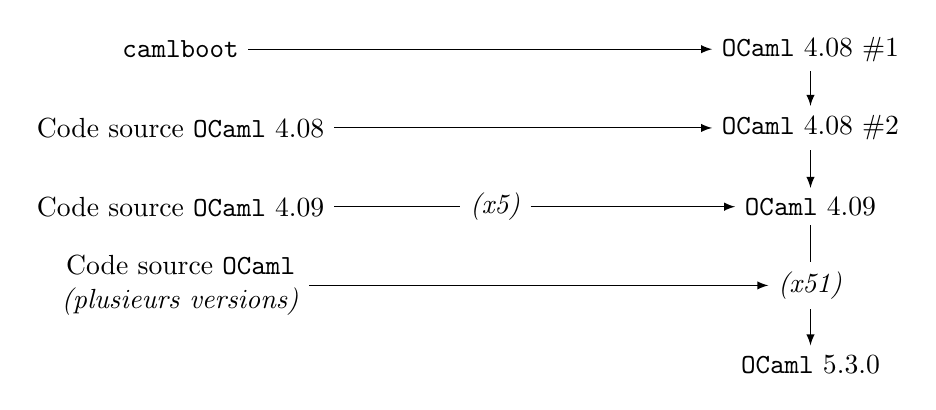
\begin{tikzpicture}
            \node (camlboot) at (-4, 0) {\texttt{camlboot}};
            \node (ocaml_408_1) at (4, 0) {\texttt{OCaml} 4.08 \#1};

            \draw[-latex] (camlboot.east) to (ocaml_408_1.west);

            \uncover<2->{
                \node (ocaml_408_source) at (-4, -1) {Code source \texttt{OCaml} 4.08};
                \node (ocaml_408_2) at (4, -1) {\texttt{OCaml} 4.08 \#2};

                \draw[-latex] (ocaml_408_source.east) to (ocaml_408_2.west);
                \draw[-latex] (ocaml_408_1.south) to (ocaml_408_2.north);
            }

            \uncover<3->{
                \node (ocaml_409_source) at (-4, -2) {Code source \texttt{OCaml} 4.09};
                \node (409_iterations) at (0, -2) {\emph{(x5)}};
                \node (ocaml_409) at (4, -2) {\texttt{OCaml} 4.09};

                \draw (ocaml_409_source.east) to (409_iterations.west);
                \draw[-latex] (409_iterations.east) to (ocaml_409.west);
                \draw[-latex] (ocaml_408_2.south) to (ocaml_409.north);
            }

            \uncover<4->{
                \node (ocaml_530) at (4, -4) {\texttt{OCaml} 5.3.0};
                \node (ocaml_530_iterations) at (4, -3) {\emph{(x51)}};
                \node[align=center] (ocaml_source) at (-4, -3) {
                    Code source \texttt{OCaml} \\
                    \emph{(plusieurs versions)}
                };

                \draw (ocaml_409.south) to (ocaml_530_iterations.north);
                \draw[-latex] (ocaml_530_iterations.south) to (ocaml_530.north);
                \draw[-latex] (ocaml_source.east) to (ocaml_530_iterations.west);
            }
        \end{tikzpicture}
    \end{center}
\end{frame}

\subsection{Bootstrapping du projet camlboot}
\begin{frame}
    \frametitle{Bootstrapping du projet camlboot\esp}

    \begin{center}
        \begin{tikzpicture}
            \node (camlboot) at (-3, 0.5) {
                \texttt{camlboot}
            };
            \node (ocaml_408) at (3, 0.5) {\texttt{OCaml} 4.08};

            \draw[-latex] (camlboot.east) to (ocaml_408.west);

            \uncover<2->{
                \node (gcc) at (-3, -1) {\boxed{\texttt{gcc}}};
            }

            \uncover<3->{
                \node[align=center] (miniml_compiler) at (3, -2.2) {
                    \texttt{miniml/compiler} \\
                    \emph{\'Ecrit en Scheme}
                };

                \node[align=center] (miniml_interp) at (3, -3.4) {
                    \texttt{miniml/interp} \\
                    \emph{\'Ecrit en OCaml}
                };

                \node[draw,dashed,fit=(miniml_compiler) (miniml_interp)] (camlboot_inner) {};
            }

            \uncover<4->{
                \node[align=center] (guile) at (3, -1) {
                    \texttt{Guile} \emph{(Scheme)} \\
                    \emph{\'Ecrit en C}
                };
            }

            \uncover<5->{
                \node[align=center] (ocamlc) at (3, -4.6) {
                    \texttt{ocamlc} \\
                    \emph{\'Ecrit en OCaml}
                };
            }

            \uncover<6->{
                \node[align=center] (ocaml_source) at (-3, -4.6) {
                    Autres composantes \texttt{OCaml} \\
                    \emph{\'Ecrits en C et OCaml}
                };

                \node (ocaml_408_inner) at (-3, -5.8) {\texttt{OCaml} 4.08};
            }

            \node (marker_left) at (-5, -1) {};
            \node (marker_right) at (5, -1) {};

            \uncover<3->{
                \draw[-latex] (miniml_compiler.south) to (miniml_interp.north);
            }

            \uncover<3>{
                \draw[-latex] (gcc.east) to node[above] {?} (camlboot_inner.west);
            }

            \uncover<4->{
                \draw[-latex] (gcc.east) to (guile.west);
                \draw[-latex] (guile.south) to (miniml_compiler.north);
            }

            \uncover<5->{
                \draw[-latex] (miniml_interp.south) to (ocamlc.north);
            }

            \uncover<6->{
                \draw[-latex] (gcc.south) to (ocaml_source.north);
                \draw[-latex] (ocamlc.west) to (ocaml_source.east);
                \draw[-latex] (ocaml_source.south) to (ocaml_408_inner.north);
            }

            \uncover<2->{
                \node[draw,fit=(marker_left) (marker_right) (miniml_compiler) (miniml_interp) (ocamlc) (ocaml_source) (guile) (gcc) (ocaml_408_inner)] {};
            }
        \end{tikzpicture}
    \end{center}
\end{frame}

\subsection{Bootstrapping du C}
\begin{frame}
    \frametitle{Bootstrapping du C\esp}
    \begin{center}
        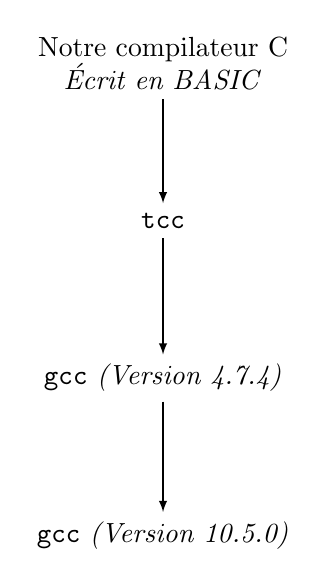
\begin{tikzpicture}
            \node[align=center] (our_compiler) at (0, 0) {
                Notre compilateur C \\
                \emph{\'Ecrit en BASIC}
            };

            \uncover<2->{
                \node (tcc) at (0, -2) {\boxed{\texttt{tcc}}};
                \draw[-latex] (our_compiler.south) to (tcc.north);
            }

            \uncover<3->{
                \node (gcc_474) at (0, -4) {\boxed{\texttt{gcc}} \emph{(Version 4.7.4)}};
                \draw[-latex] (tcc.south) to (gcc_474.north);
            }

            \uncover<4->{
                \node (gcc_1050) at (0, -6) {\boxed{\texttt{gcc}} \emph{(Version 10.5.0)}};
                \draw[-latex] (gcc_474.south) to (gcc_1050.north);
            }
        \end{tikzpicture}
    \end{center}
\end{frame}

\subsection{R\'esultats}
\begin{frame}
    \frametitle{R\'esultats\esp}

    \begin{center}
        \begin{tikzpicture}
            \node (our_compiler) {Notre compilateur C};
            \node[right=0.3cm of our_compiler] (tcc) {\boxed{\texttt{tcc}}};
            \node[right=0.3cm of tcc] (gcc) {\boxed{\texttt{gcc}}};
            \node[right=0.3cm of gcc] (guile) {\texttt{Guile}};
            \node[right=0.3cm of guile] (camlboot) {\texttt{camlboot}};
            \node[right=0.3cm of camlboot] (ocaml) {\texttt{OCaml}};

            \draw[-latex] (our_compiler.east) to (tcc.west);
            \draw[-latex] (tcc.east) to (gcc.west);
            \draw[-latex] (gcc.east) to (guile.west);
            \draw[-latex] (guile.east) to (camlboot.west);
            \draw[-latex] (camlboot.east) to (ocaml.west);
        \end{tikzpicture}
    \end{center}

    \uncover<2->{
        \vspace{0.5cm}

        Pour compiler le programme suivant:

        \mint{ocaml}|print_endline "Hello, World!";;|

        \vspace{0.5cm}
    }

    \uncover<3->{
        \begin{itemize}
            \item XX heures de compilation
                  \uncover<4->{
            \item XX de fichiers g\'en\'er\'es \`a partir de XX de fichiers source
                  }
        \end{itemize}
    }

    \uncover<5->{
        \vspace{0.5cm}

        Mais...

        \begin{itemize}
            \item Une garantie quant \`a la sécurité de l'ex\'ecutable produit
                  \uncover<6->{
            \item Une preuve que le projet \texttt{OCaml} est reconstructible \`a
                  partir d'archives.
                  }
        \end{itemize}
    }
\end{frame}
